\chapter{Domain}
\label{chap:domain}

This chapter begins with an high level description of the domain. This is followed by a description of the schema in the relational database of CIMS.
\begin{figure}[h!]
\centering
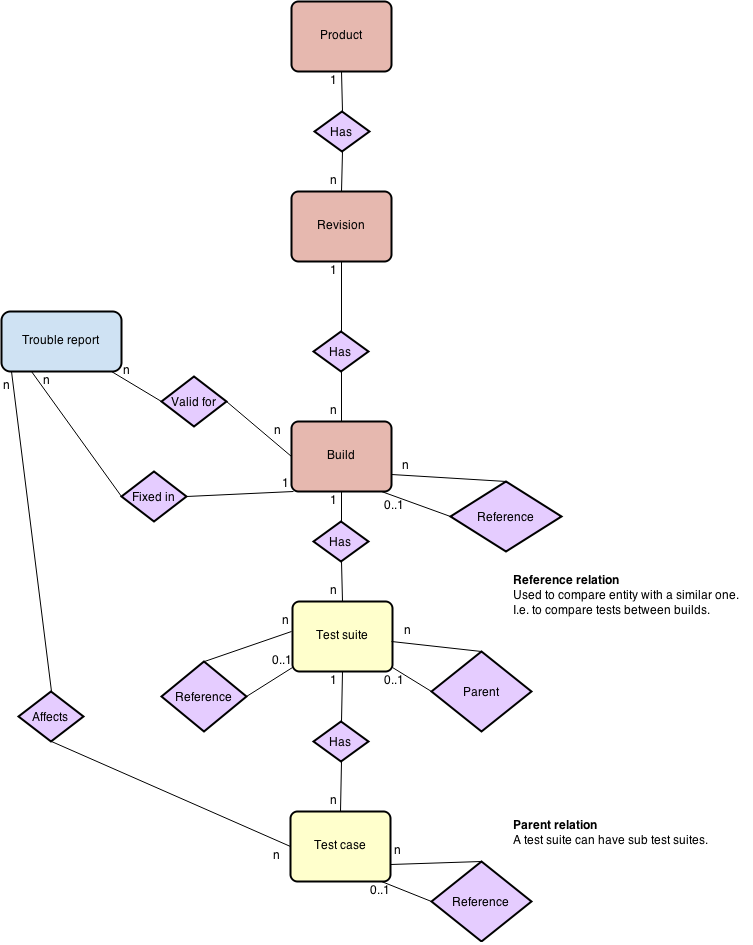
\includegraphics[scale=0.5]{figure/er_diagram.png}
\caption{High level diagram of the domain.}
\label{fig:er}
\end{figure}

\section{Description}
The domain in which CIMS operates has the following high level entities; products, revisions, builds, test suites, test cases and trouble reports. Excluding trouble reports, these entities form a hierarchical structure as seen in figure~\ref{fig:er}. Products are at the top of this hierarchy. They represent the different software systems that are being developed at Ericsson. Products are developed iteratively, where each released iteration is called a revision. At the revision level, developers makes changes to source code, configuration, tests etc.\ which are then checked into a revision control system and subsequently built and tested. This is referred to in domain terms as a build. Each build runs a number of test suites, which in turn consist of a number test cases.

As has been noted, a trouble report sits outside of the hierarchy. This entity represents a bug or defect which arrives from external (i.e.\ a customer) or internal sources. It can be mapped to different entities from products down to specific test cases. Trouble reports are handled by implementing a fix in a specific build.

\section{Database schema}
The relational database schema in use by CIMS represents the above mentioned entities in a different abstraction. Representation of these entCrowities are described in depth in the sections below.
The schema of the relational database in CIMS is presented in figure~\ref{fig:sql}.

\subsection{Test suite}
\begin{figure}[h!]
\centering
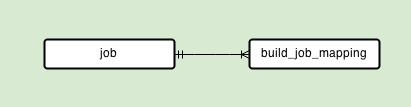
\includegraphics[scale=0.5]{figure/job.png}
\caption{Diagram of tables related to test suites using Crow's foot notation.}
\label{fig:job}
\end{figure}
The top level entity of a test suite is represented by the job table. A job is used to group job\_events   . As seen in figure~\ref{fig:job}, a job belongs to a build via the build\_job\_mapping table.   
\subsection{Build}
\begin{figure}[h!]
\centering
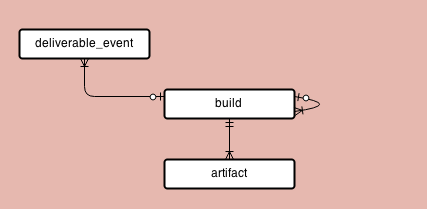
\includegraphics[scale=0.5]{figure/build.png}
\caption{Diagram of tables related to builds.}
\label{fig:build}
\end{figure}
\subsection{Test case}
\begin{figure}[h!]
\centering
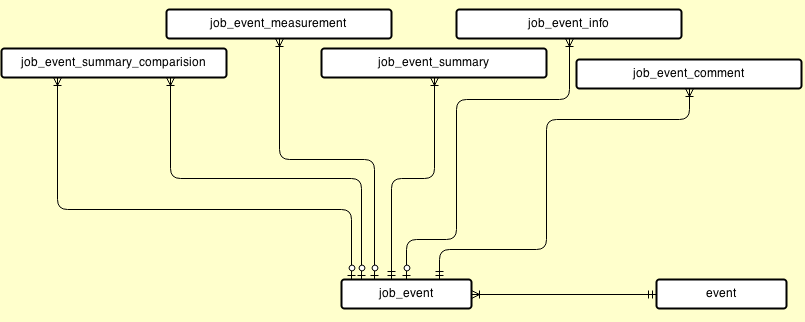
\includegraphics[scale=0.5]{figure/job_event.png}
\caption{Diagram of tables related to test cases.}
\label{fig:job_event}
\end{figure}
\subsection{Deliverable}
\begin{figure}[h!]
\centering
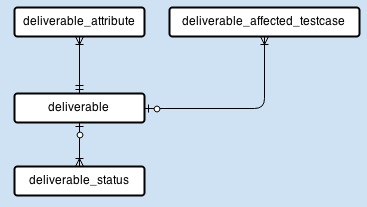
\includegraphics[scale=0.5]{figure/deliverable.png}
\caption{Diagram of tables related to trouble reports.}
\label{fig:deliverable}
\end{figure}






\section{Data influx}

The organization is always improving their continuous integration process, which leads to shorter lead times in the building process of a software. This leads to that more and more builds that are being registered in CIMS. During the CIMS lifetime, the influx of job events can be seen in ~\ref{fig:jeTrend}. This figure clearly shows the trend in the data inflow of CIMS, it is far from linear. The trend is hitherto increasing, there are many factors involved in describing the origin of this trend. Shorter lead times, organization more experienced with CIMS, Agile, LEAN.

\begin{figure}[h!]
\centering
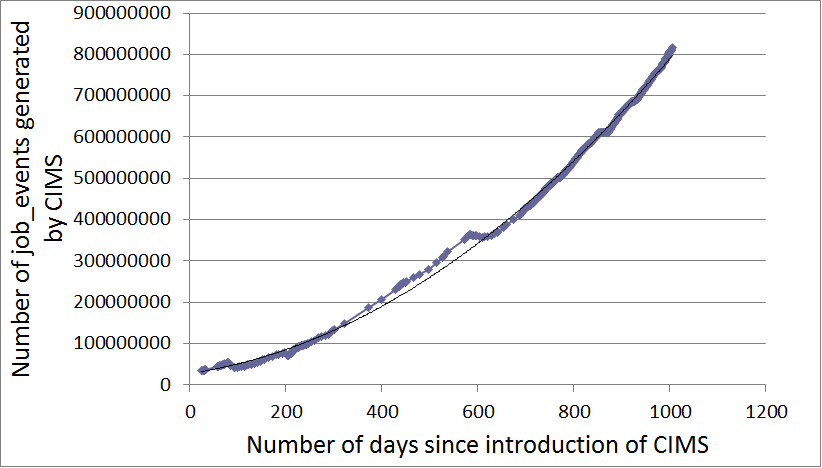
\includegraphics[scale=0.65]{figure/jeTrends.png}
\caption{Diagram showing the inflow of data into CIMS.}
\label{fig:jeTrend}
\end{figure}

\section{Use cases}
The set of important queries that the archive should support is presented in table~\ref{tab:queries}.

TODO: Detailed textual description of the queries.

\begin{figure}[h!]
\centering
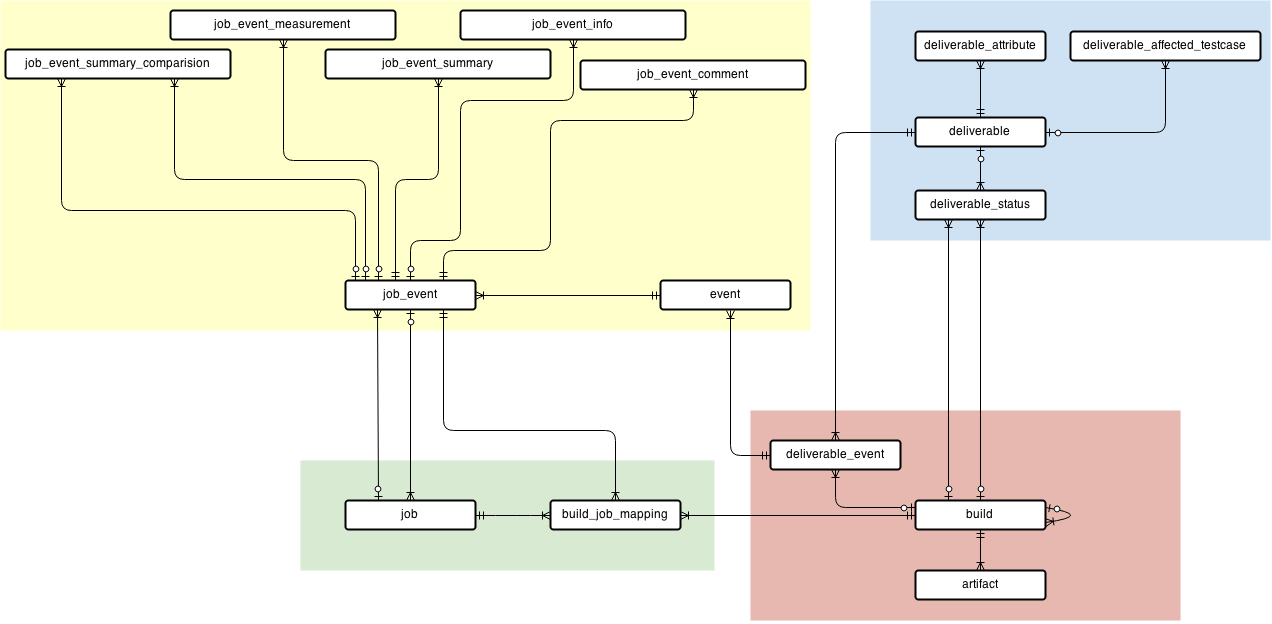
\includegraphics[scale=0.5, angle=90]{figure/sql.png}
\caption{Diagram of the relational database in CIMS using Crow's foot notation.}
\label{fig:sql}
\end{figure}

\begin{table}[h]
\begin{tabular}{|l|l|}
\hline
\textbf{High level query}                & \textbf{Query in CIMS}                    \\ \hline
Get build                                    & Get build by id                           \\ \hline
Get build information                        & Get build information by id               \\ \hline
Get build for root test suite                & Get build by simple id                    \\ \hline
Get trouble reports for build                & Get deliverables for build                \\ \hline
Get trouble report fixes for build           & Get deliverables for build                \\ \hline
Get trouble reports for product and revision & Get deliverables for product and revision \\ \hline
Get test suite children                      & Get job event children                    \\ \hline
Get test case in build                       & Get job event by id                       \\ \hline
Get test suite in build                      & Get job event by id                       \\ \hline
Get root test suite for test case/test suite & Get root job event                        \\ \hline
Get test case by name                        & Get job event by name                     \\ \hline
Get test suite for test case                 & Get parent job event                      \\ \hline
Get test case history                        & Get event history                         \\ \hline
Get test tree                                & Get job tree by id                        \\ \hline
\end{tabular}
\caption{Set of important queries on the relational database of CIMS}
\label{tab:queries}
\end{table}


%\section{Architecture of CIMS}

%CIMS has a multitier architecture as seen in figure X. Whenever a build is started, data from multiple sources is collected and sent to the system. This data is transformed to fit into the relational data model of CIMS.
%
%Presentation of data is done in real time via a web application. In order to support this, CIMS employs a number technologies in support of the main relational database, effectively forming a polyglot persistence solution. This includes a search engine (Sphinx) for aggregation of test cases, and a key value store (Redis) for caching.
%
%An external REST API is exposed to gather data for other purposes than real time visualization.